\chapter{Methodology}\label{sec:methodology}

This chapter details the empirical methodology employed to investigate the relationship between technical debt, development velocity, and funding success in venture-backed software companies during the \ac{ZIRP} era. The approach combines automated large-scale code analysis with longitudinal funding data to provide a systematic, cross-company examination of these relationships in the startup ecosystem.

\section{Research Design and Sample Construction}\label{sec:research_design}

This study employs a quantitative, longitudinal design examining 70 venture-backed companies across 146 inter-funding periods between 2009-2022. The unit of analysis is the development period between consecutive funding rounds, enabling observation of how technical debt accumulation and development velocity patterns associate with subsequent funding success. This design addresses a fundamental limitation in existing technical debt research, which has predominantly relied on single-company case studies or cross-sectional analyses of mature organizations \cite{li2015systematic}.

The longitudinal approach captures the dynamic strategic trade-offs that characterize venture-backed development. By analyzing the same companies across multiple funding cycles, the design helps isolate the relationship between technical execution patterns and market validation through investor decisions.

\begin{figure}[htbp]
\centering
\begin{tikzpicture}[node distance=0.8cm and 1.2cm, scale=0.9, transform shape]
    % Define colors
    \definecolor{datacolor}{RGB}{52, 152, 219}
    \definecolor{processcolor}{RGB}{39, 174, 96}
    \definecolor{analysiscolor}{RGB}{243, 156, 18}
    \definecolor{outputcolor}{RGB}{231, 76, 60}
    
    % Data Sources (stacked vertically)
    \node[draw, thick, fill=datacolor!20, text width=1.8cm, align=center, minimum height=0.8cm] (startup_data) {
        \textbf{Startup DB}
    };
    
    \node[draw, thick, fill=datacolor!20, text width=1.8cm, align=center, minimum height=0.8cm, below=0.2cm of startup_data] (github_data) {
        \textbf{GitHub}\\
        \small Repos
    };
    
    % Filtering
    \node[draw, thick, fill=processcolor!20, text width=2cm, align=center, minimum height=1.3cm, right=0.8cm of startup_data, yshift=-0.8cm] (filtering) {
        \textbf{Filtering}\\
        \small ZIRP era\\
        \small Series A\\
        \small Open source
    };
    
    % Pipeline
    \node[draw, thick, fill=analysiscolor!20, text width=2cm, align=center, minimum height=1.3cm, right=0.8cm of filtering] (pipeline) {
        \textbf{Pipeline}\\
        \small Automated\\
        \small analysis
    };
    
    \node[draw, thick, fill=analysiscolor!20, text width=1.7cm, align=center, minimum height=0.8cm, right=0.8cm of pipeline, yshift=1cm] (tdr_calc) {
        \textbf{TDR}\\
        \small COCOMO
    };
    
    \node[draw, thick, fill=analysiscolor!20, text width=1.7cm, align=center, minimum height=0.8cm, right=0.8cm of pipeline, yshift=-1cm] (velocity_calc) {
        \textbf{Velocity}\\
        \small Composite
    };
    
    % Final outputs
    \node[draw, thick, fill=outputcolor!20, text width=2cm, align=center, minimum height=1cm, right=0.8cm of tdr_calc, yshift=-1cm] (final_sample) {
        \textbf{Dataset}\\
        \small 70 companies\\
        \small 146 periods
    };
    
    \node[draw, thick, fill=outputcolor!20, text width=2.2cm, align=center, minimum height=1cm, right=0.8cm of final_sample] (analysis) {
        \textbf{Analysis}\\
        \small Correlation\\
        \small Strategic framework
    };
    
    % Arrows - horizontal flow
    \draw[thick, ->] (startup_data) -- (filtering);
    \draw[thick, ->] (github_data) -- (filtering);
    \draw[thick, ->] (filtering) -- (pipeline);
    \draw[thick, ->] (pipeline) -- (tdr_calc);
    \draw[thick, ->] (pipeline) -- (velocity_calc);
    \draw[thick, ->] (tdr_calc) -- (final_sample);
    \draw[thick, ->] (velocity_calc) -- (final_sample);
    \draw[thick, ->] (final_sample) -- (analysis);
    
\end{tikzpicture}
\caption{Research Methodology Overview}
\label{fig:methodology_overview}
\end{figure}

\subsection{Population Definition and Systematic Filtering}

Sample construction began with an initial population of venture capital-backed software companies identified through comprehensive database searches of Crunchbase and Tracxn. This population underwent systematic filtering to ensure analytical rigor and theoretical relevance.

The temporal filtering criterion required companies to have raised Series A funding during the ZIRP era (2009-2022). Data suggests a typical timeframe of 12-24 months between funding rounds for venture-backed companies \cite{gornall2020squaring}. To ensure sufficient time for a subsequent round to be evaluated, a cutoff was established requiring at least 36 months between the Series A date and the data collection point. Series A represents a critical validation milestone where companies are expected to have demonstrated product-market fit beyond initial seed-stage experiments, making it an appropriate baseline for examining development practices under venture pressure \cite{sahlman1990structure}.

All funding information was cross-validated using Crunchbase and Tracxn databases. The open-source requirement, while a limitation on generalizability, was necessary to enable the comprehensive code analysis for technical debt measurement. Companies were included only when their primary product codebase was publicly accessible.

The remaining companies were classified into six industry categories: 

\begin{table}[h]
\centering
\caption{Distribution of Companies by Industry Category}
\label{tab:industry_distribution}
\begin{tabular}{lc}
\hline
\textbf{Industry Category} & \textbf{Count} \\
\hline
Developer Tools \& DevOps & 23 \\
Database \& Storage & 18 \\
Data Platform \& Analytics & 12 \\
Business \& Application Software & 8 \\
Security & 5 \\
AI/Machine Learning & 4 \\
\hline
\end{tabular}
\end{table}

Further technical filtering was applied to ensure the quality of the data. A minimum threshold of 5,000 average lines of code across observation periods was required to ensure that \ac{TDR} calculations reflect substantial software systems rather than early prototypes. Additionally, development periods shorter than 90 days were removed to avoid noise from insignificant development activity.

This comprehensive filtering process reduced an initial set of 153 potential development periods to a final analytical sample of 146 periods from 70 companies, yielding a data retention rate of 95.4\%. This process balances the need for a sufficiently large sample with the requirements of data quality for robust analysis.

\section{Data Collection and Measurement Procedures}\label{sec:data_collection}

This section details the automated analysis pipeline and the specific methodologies for measuring technical debt and development velocity. The approach combines novel automation techniques with established measurement frameworks to enable large-scale, objective analysis.

\subsection{Automated Analysis Pipeline}\label{sec:analysis_pipeline}

A core component of this research is a novel, automated pipeline that synchronizes funding timeline data with historical code repository states. This pipeline addresses the challenge of measuring technical debt as it existed at the point of investor decision-making.

For each company, the pipeline clones the primary product repository. To align with the venture capital due diligence process, which evaluates a company's state leading up to an investment decision \cite{sahlman1990structure}, the analysis pipeline checks out the repository to the commit state closest to, but not after, each funding announcement date. This ensures that technical debt measurements reflect the code quality available to investors during their evaluation.

The repository states are then analyzed using the Qlty CLI platform. This tool was selected over other static analysis tools, such as SonarQube, due to its documented performance on large-scale codebases and its suitability for analyzing the varied projects in the sample. The pipeline manages Qlty execution across multiple repositories while handling memory constraints and timeout issues. The complete technical implementation is detailed in Appendix~\ref{app:technical_implementation}.

\subsection{Static Analysis Tool Selection and Validation}

The selection of appropriate static analysis tools represents a critical methodological decision that directly impacts the validity and generalizability of technical debt measurements. This subsection details the systematic evaluation process used to select Qlty CLI as the primary analysis platform and addresses the implications of tool-specific measurement characteristics.

\begin{table}[htbp]
\centering
\caption{Comparative Analysis of Static Analysis Platforms for Cross-Company Research}
\label{tab:static_analysis_methodology}
\begin{tabular}{|p{2.8cm}|p{3.8cm}|p{3.5cm}|p{4.4cm}|}
\hline
\textbf{Platform} & \textbf{Primary Focus} & \textbf{TDR Approach} & \textbf{Research Suitability} \\
\hline
\textbf{SonarQube} & 
Continuous inspection of code quality, security, and reliability for development teams & 
Time-based remediation cost using default development rates (e.g., 30 min/KLOC) & 
\textbf{High:} Open-source availability, extensive language support, standardized metrics, strong API access \\
\hline
\textbf{CAST} & 
Portfolio-level analysis of software health and structural risk for enterprise systems & 
Business impact-focused debt calculation prioritizing high-risk structural flaws & 
\textbf{Medium:} Comprehensive analysis but proprietary algorithms, limited academic access \\
\hline
\textbf{Qlty (CodeClimate successor)} & 
Multi-language static analysis with configurable rule sets for large-scale codebases & 
Effort-based remediation cost calculation with detailed issue categorization & 
\textbf{High:} Scalable CLI interface, consistent cross-language analysis, suitable for automated research pipelines \\
\hline
\end{tabular}
\end{table}

Qlty CLI was selected based on three primary criteria relevant to large-scale cross-company analysis: scalability for automated processing of diverse codebases, consistency of output formatting across different programming languages, and transparency of remediation cost calculations that enable reproducible \ac{TDR} computation. The platform's command-line interface proved essential for the automated pipeline developed for this research, enabling batch processing of repository states synchronized with funding timeline data.

However, the selection of any single static analysis tool introduces systematic measurement limitations that must be acknowledged. Empirical studies document significant divergence between tools when analyzing identical codebases, with overlap in identified issues typically less than 15\% \citep{wang2018comprehensive}. Additionally, precision rates vary considerably, ranging from 20\% to 80\% depending on configuration \citep{beller2016analyzing}. These inter-tool variations mean that \ac{TDR} measurements become tool-specific rather than universally generalizable, establishing an important boundary condition for the interpretation of empirical relationships observed in this study.

The tool-specific measurement characteristics have direct implications for the strategic framework developed in this research. Companies classified as ``high debt'' based on Qlty analysis may receive different classifications from alternative static analysis platforms, suggesting that the strategic quadrants identified represent patterns specific to code-level issues detected by Qlty's rule sets rather than comprehensive assessments of technical health across all debt dimensions.

\subsection{Technical Debt Ratio Implementation and Economic Modeling}
Technical debt is quantified using the \ac{TDR} framework, which provides an economic interpretation of code quality relevant to the financial context of venture capital evaluation. As defined in the literature review, \ac{TDR} represents the ratio of remediation cost to total estimated development cost, enabling direct comparison of quality trade-offs across companies with different codebase sizes and development investments.

The remediation cost component is derived from the `totalEffortMinutes` metric produced by Qlty analysis. This metric estimates the developer time required to address identified structural issues, coding standard violations, and complexity problems. The effort estimation is not based on traditional complexity metrics like Cyclomatic Complexity, but is instead grounded in the principles of Cognitive Complexity \citep{Campbell2023CognitiveComplexity}. Cognitive Complexity is a modern metric designed to measure the understandability of code from a human perspective, penalizing structures that break the linear flow of code and require greater mental effort to comprehend, such as nested control flows and complex logical expressions. Qlty translates these principles into a quantifiable remediation cost by assigning a baseline effort in minutes to each type of issue (`BASE\_EFFORT\_MINUTES`) and adding an incremental penalty based on the severity of the issue (`EFFORT\_MINUTES\_PER\_VALUE\_DELTA`). This approach reflects the platform's assessment of the ``interest payments'' associated with current technical debt levels—the additional development time required for future modifications due to existing quality constraints.

The development cost denominator employs the Basic \ac{COCOMO} model's organic mode for standardized cost estimation across the dataset. \ac{COCOMO} estimates development effort as $E = a \times (KLOC)^b$, where the organic mode parameters ($a = 2.4$, $b = 1.05$) are specifically designed for small-to-medium software projects with stable requirements and experienced teams—characteristics that closely match the venture-backed startup environment analyzed in this study. The organic mode's lower complexity exponent (1.05) reflects the relatively straightforward development challenges typical of early-stage software companies, making it the most appropriate \ac{COCOMO} variant for this research context.

Crucially, while \ac{COCOMO}'s absolute cost predictions exhibit documented variability in individual projects \citep{jeklin2025evaluation}, the model's strength lies in providing consistent relative estimates across organizations—precisely what is required for \ac{TDR} calculation. The systematic application of identical parameters across all 70 companies ensures that observed differences in technical debt ratios reflect genuine variations in code quality rather than estimation inconsistencies. This methodological consistency enables the cross-company comparative analysis that forms the foundation of this research.

The \ac{TDR} implementation acknowledges that the ratio primarily captures code-level debt detected by static analysis, potentially excluding architectural, test, and documentation debt that may influence startup velocity. However, code-level debt represents the most objectively measurable and comparable form of technical debt across organizations, providing a standardized foundation for empirical analysis. The economic framing through \ac{COCOMO} enables direct comparison of quality investments across companies with different scales and development histories.

For the large-scale empirical analysis undertaken in this research, \ac{TDR} provides the optimal balance of objective measurement, cross-company comparability, and theoretical grounding necessary to examine technical debt relationships in venture-backed environments. The consistent application of organic mode \ac{COCOMO} parameters ensures that strategic insights emerge from genuine patterns in the data rather than methodological artifacts.


\subsection{Theoretical Justification for TDR as Strategic Proxy}

While \ac{TDR} calculations capture code-level manifestations of quality trade-offs, interpreting these patterns as evidence of strategic choices requires establishing theoretical connections between observable technical metrics and organizational decision-making processes. This theoretical foundation justifies using \ac{TDR} patterns as proxies for startup strategic priorities rather than treating them as merely technical artifacts.

The theoretical bridge from code metrics to strategic intent rests on three complementary frameworks. First, resource allocation theory from organizational behavior \citep{cyert1963behavioral} explains that consistent patterns of code-level debt across multiple modules and development periods reflect systematic organizational choices rather than random technical accidents. When teams repeatedly choose expedient implementations over architectural elegance across diverse technical contexts, these patterns reveal underlying resource allocation priorities embedded in organizational culture and incentive structures.

Second, applying behavioral signal theory \citep{spence1973job} to the technical debt context, code-level debt accumulation patterns serve as observable indicators of organizational risk tolerance and temporal preferences. Teams that consistently accept higher complexity and defer quality improvements across multiple development cycles reveal their strategic orientation toward short-term achievement over long-term sustainability. Unlike traditional signaling contexts where agents actively manage their signals, technical debt patterns represent authentic behavioral indicators that emerge from genuine organizational priorities.

Third, constraint-based decision making literature \citep{simon1955behavioral} provides the economic rationality for systematic debt accumulation as optimal strategic choice. In venture-backed environments characterized by severe time constraints and competitive pressures, technical debt represents ``temporal arbitrage''—systematically trading future development capacity for immediate execution capability when current capacity is more valuable than equivalent future capacity \citep{fisher1930theory}.

This theoretical convergence establishes \ac{TDR} as a valid proxy for organizational strategic intent regarding quality-speed trade-offs, enabling interpretation of observed empirical relationships as evidence of strategic rather than merely technical phenomena.

\subsection{Composite Velocity Framework}

Development velocity is measured using the composite metric defined in \autoref{eq:composite-velocity}, adapted from the CNCF's project velocity framework for the startup evaluation context. 

The implementation extracts the required components from Git repository data for each development period. Code churn per author is calculated by summing lines added and deleted, normalized by period length and team size. Commits per author represents the development rhythm over the same normalized basis. Both metrics are then scaled by their respective dataset maximums to ensure the composite velocity ranges from 0 to 1, enabling meaningful cross-company comparison despite significant variations in team sizes across venture-backed startups.

The per-author normalization accounts for teams within the sample, while the max-normalization ensures that companies with different absolute activity levels can be meaningfully compared on execution intensity.

\section{Statistical Challenges and Solutions}\label{sec:statistical_challenges}

A fundamental challenge in this longitudinal study is the nested structure of the data and ensuring appropriate statistical inference. This section addresses the key statistical issues and presents the solutions employed to maintain analytical rigor.

\subsection{Addressing the Nested Data Structure Problem}

The dataset contains 146 development periods from 70 companies, meaning that some companies contribute multiple observations. This structure violates the independence assumption underlying standard correlation and regression analyses, as observations from the same company are likely to be correlated due to consistent organizational practices, team capabilities, and strategic approaches \citep{raudenbush2002hierarchical}.

To address this statistical validity concern, this study employs a dual analytical approach that provides both granular and aggregate perspectives on the relationships of interest:

\textbf{Per-Period Analysis}: The primary descriptive analysis examines correlations across all 146 individual development periods, providing detailed insight into period-to-period variations in technical debt and velocity patterns. While this approach maximizes statistical power and captures the full range of strategic transitions within companies, it acknowledges that the independence assumption may be violated.

\textbf{Per-Company Analysis}: To ensure statistical validity, a complementary analysis aggregates all metrics to the company level by calculating mean values across all periods for each company. This approach transforms the nested structure into 70 independent company-level observations, satisfying the independence assumption required for correlation analysis. The per-company analysis serves as the primary basis for statistical inference, while the per-period analysis provides additional descriptive insight.

The implementation calculates company-level averages as:

\vspace{-0.8cm}

\begin{align}
\text{For each company } c \text{ with periods } p_1, p_2, \ldots, p_n: \nonumber \\
\overline{\text{TDR}}_c &= \frac{1}{n} \sum_{i=1}^{n} \text{TDR}_{p_i} \\
\overline{\text{Velocity}}_c &= \frac{1}{n} \sum_{i=1}^{n} \text{Velocity}_{p_i} \\
\overline{\text{FundingGrowth}}_c &= \frac{1}{n} \sum_{i=1}^{n} \text{FundingGrowth}_{p_i}
\end{align}

This dual approach allows for robust statistical inference while preserving the rich longitudinal information captured in the dataset.

\subsection{Statistical Power and Inference Procedures}

For both the per-period and per-company analyses, statistical significance is assessed using Pearson correlation coefficients with associated p-values calculated using the t-distribution. The degrees of freedom are adjusted appropriately: $n-2$ for the per-period analysis (144 degrees of freedom) and $c-2$ for the per-company analysis (68 degrees of freedom), where $c$ represents the number of companies.

Given the exploratory nature of this research and the relatively novel application domain, significance levels are interpreted using conventional thresholds ($p < 0.05$ for significance, $p < 0.10$ for marginal significance) while emphasizing effect sizes and practical significance alongside statistical significance.

The regression analysis provides $R^2$ values to quantify the proportion of variance in development velocity explained by technical debt levels, offering insight into both the statistical and practical importance of the relationship.

\section{Strategic Framework and Analysis Approaches}\label{sec:strategic_framework}

Beyond examining simple correlations, this study develops a strategic framework for understanding technical debt and velocity combinations. This section details the multi-framework approach used to test the robustness of strategic insights across different analytical perspectives.

\subsection{Primary Strategic Framework: The Debt-Velocity Matrix}

The core analytical framework classifies companies into four strategic quadrants based on their technical debt and development velocity profiles. This matrix provides a practical tool for understanding the strategic implications of different debt-velocity combinations in venture-backed environments.

\begin{figure}[htbp]
\centering
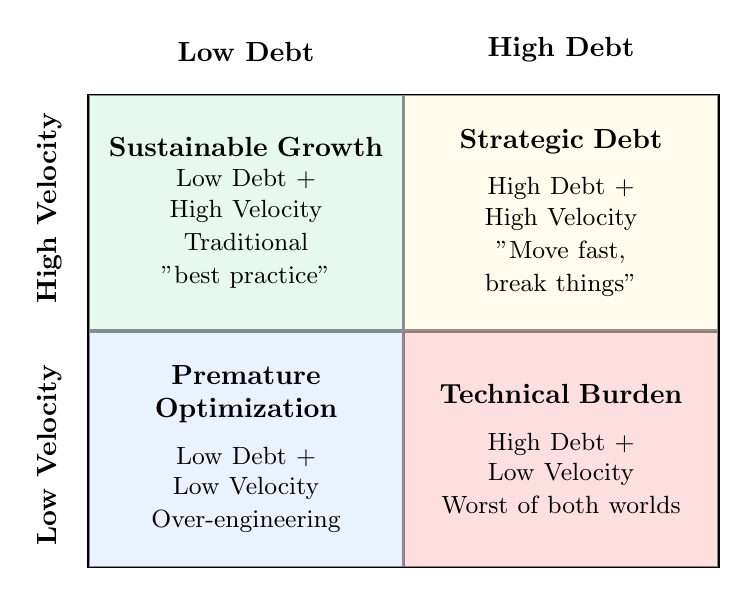
\begin{tikzpicture}[scale=1]
    % Define colors
    \definecolor{sustainable}{RGB}{213, 244, 230}
    \definecolor{strategic}{RGB}{255, 248, 225}
    \definecolor{premature}{RGB}{219, 234, 254}
    \definecolor{burden}{RGB}{254, 202, 202}
    
    % Draw the main axes
    \draw[very thick] (-4,0) -- (4,0);
    \draw[very thick] (0,-3) -- (0,3);
    
    % Draw quadrant boxes
    \draw[thick] (-4,-3) rectangle (0,0);  % Bottom-left
    \draw[thick] (0,-3) rectangle (4,0);   % Bottom-right
    \draw[thick] (-4,0) rectangle (0,3);   % Top-left
    \draw[thick] (0,0) rectangle (4,3);    % Top-right
    
    % Fill quadrants with colors
    \fill[sustainable, opacity=0.6] (-4,0) rectangle (0,3);    % Top-left: Sustainable Growth
    \fill[strategic, opacity=0.6] (0,0) rectangle (4,3);     % Top-right: Strategic Debt
    \fill[premature, opacity=0.6] (-4,-3) rectangle (0,0);   % Bottom-left: Premature Optimization
    \fill[burden, opacity=0.6] (0,-3) rectangle (4,0);      % Bottom-right: Technical Burden
    
    % Axis labels
    \node[above] at (-2,3.3) {\textbf{Low Debt}};
    \node[above] at (2,3.3) {\textbf{High Debt}};
    
    \node[left, rotate=90] at (-4.5,2.9) {\textbf{High Velocity}};
    \node[left, rotate=90] at (-4.5,-0.3) {\textbf{Low Velocity}};
    
    % Quadrant content - Top-left
    \node[text width=3.5cm, align=center] at (-2,1.5) {
        \textbf{Sustainable Growth}\\
        \small Low Debt + High Velocity\\
        \small Traditional "best practice"
    };
    
    % Quadrant content - Top-right
    \node[text width=3.5cm, align=center] at (2,1.5) {
        \textbf{Strategic Debt}\\[0.2cm]
        \small High Debt + High Velocity\\
        \small "Move fast, break things"
    };
    
    % Quadrant content - Bottom-left
    \node[text width=3.5cm, align=center] at (-2,-1.5) {
        \textbf{Premature Optimization}\\[0.2cm]
        \small Low Debt + Low Velocity\\
        \small Over-engineering
    };
    
    % Quadrant content - Bottom-right
    \node[text width=3.5cm, align=center] at (2,-1.5) {
        \textbf{Technical Burden}\\[0.2cm]
        \small High Debt + Low Velocity\\
        \small Worst of both worlds
    };
    
\end{tikzpicture}
\caption{Strategic Framework: Technical Debt-Velocity Matrix}
\label{fig:strategic_framework}
\end{figure}

The four strategic quadrants are defined as:

\textbf{Sustainable Growth (Low Debt + High Velocity)}: Companies that achieve high development velocity while maintaining low technical debt levels. This represents the traditional engineering ideal of sustainable, high-quality development practices.

\textbf{Strategic Debt (High Debt + High Velocity)}: Companies that accept high technical debt levels in pursuit of maximum development velocity. This quadrant embodies the "move fast and break things" philosophy and represents the key strategic question of this research.

\textbf{Premature Optimization (Low Debt + Low Velocity)}: Companies with low technical debt but also low development velocity, potentially indicating over-engineering or analysis paralysis that constrains execution speed.

\textbf{Technical Burden (High Debt + Low Velocity)}: Companies suffering from both high technical debt and low velocity, representing the worst-case scenario where debt accumulation has begun to significantly constrain development capability.

\subsection{Comprehensive Sensitivity Analysis Framework}

To ensure the robustness of findings across different statistical methodologies, this study implements a comprehensive sensitivity analysis that tests the strategic framework using multiple classification approaches. This addresses potential concerns that results might be artifacts of the specific median-split methodology initially employed.

\textbf{Primary Framework (Median Split)}: Companies are classified into four strategic quadrants based on median splits of technical debt ratio and development velocity. This approach ensures balanced group sizes and provides clear strategic interpretations.

\textbf{Tertile Framework (3×3 Matrix)}: To test for non-linear relationships and provide more granular strategic categories, the analysis implements a nine-quadrant framework using tertile splits. This approach divides each metric into Low (bottom 33\%), Medium (middle 33\%), and High (top 33\%) categories, creating nine distinct strategic positions:

\begin{itemize}
    \item Low Debt × \{Low, Medium, High\} Velocity
    \item Medium Debt × \{Low, Medium, High\} Velocity
    \item High Debt × \{Low, Medium, High\} Velocity
\end{itemize}

The tertile framework is particularly valuable for identifying whether performance relationships are monotonic or whether there are optimal ``sweet spots'' that emerge in the middle ranges of either metric.

\textbf{Quartile Extremes Framework (2×2 Focused)}: To examine the most pronounced strategic differences, this analysis compares only the extreme quartiles (bottom 25\% vs. top 25\%) for both metrics, effectively filtering out the middle 50\% of observations. This approach tests whether the relationships observed in the median split framework are driven primarily by the most extreme strategic positions or represent continuous relationships across the full range of observations.

The sensitivity analysis framework is designed to test three critical methodological assumptions:
\begin{enumerate}
    \item \textbf{Threshold Sensitivity}: Whether findings are robust to different cut-point definitions
    \item \textbf{Linearity Assumptions}: Whether relationships hold across the full distribution or only at extremes
    \item \textbf{Strategic Distinctiveness}: Whether intermediate positions show meaningfully different patterns from extreme positions
\end{enumerate}

\section{Validation and Quality Assurance}\label{sec:validation}

This section consolidates the various approaches used to ensure the reliability and validity of the findings, including cross-framework validation, outlier management, and comprehensive assessment of study limitations.

\subsection{Cross-Framework Validation}

The multiple analytical frameworks serve as internal validation mechanisms. Consistent patterns across median, tertile, and quartile methodologies provide evidence that findings are not artifacts of specific analytical choices. Conversely, framework-specific results are flagged and interpreted with appropriate caution.

This validation approach is particularly important given the exploratory nature of the research questions. By demonstrating consistency across multiple analytical perspectives, the study provides greater confidence in the strategic implications derived from the data.

\subsection{Outlier Management and Sensitivity}

To ensure that results are not driven by extreme observations, the analysis implements systematic outlier detection using the \ac{IQR} method. Observations falling beyond $1.5 \times \text{IQR}$ from the first and third quartiles are identified and, where appropriate, excluded from funding growth calculations while being retained for other analyses.

The sensitivity analysis framework also serves as a natural robustness check against outlier influence, as consistent patterns across different statistical cuts suggest that findings are not dominated by a small number of extreme cases.

For transparency, all outlier exclusions are documented and their impact on key findings is explicitly tested and reported.

\subsection{Study Limitations and Mitigation Strategies}

While these methodological enhancements significantly strengthen the statistical validity of the analysis, several limitations remain:

\textbf{Sample Representativeness}: The use of open-source companies, while necessary for data access, may not be fully representative of the broader proprietary software startup ecosystem. Open-source projects often benefit from community contributions, which could influence both velocity and code quality in ways not typical for closed-source ventures \citep{colazo2010collaboration}.

\textbf{Statistical Power Trade-offs}: The per-company analysis, while statistically appropriate, reduces the effective sample size from 146 to 70 observations, potentially reducing power to detect smaller effects. This trade-off is accepted in favor of statistical validity.

\textbf{Averaging Effects}: Company-level averaging may obscure important within-company variation in strategic approaches over time. The per-period analysis preserves this information for descriptive purposes while acknowledging its statistical limitations.

\textbf{Multiple Comparison Concerns}: The use of multiple analytical frameworks increases the risk of Type I errors. Results are interpreted with awareness of this limitation, emphasizing consistency across frameworks rather than isolated significant findings.

\textbf{Confounding Variables}: The relationship between debt, velocity, and funding is likely moderated by numerous factors not fully controlled for in this analysis, such as the startup's specific industry, stage of maturity, competitive intensity, and the size and experience of the development team.

\textbf{Metric Limitations}: Both \ac{TDR} and the composite velocity metric are proxies with inherent limitations. \ac{TDR} may not capture all forms of debt, particularly architectural and strategic debt, while velocity metrics do not inherently measure the market value or strategic importance of the features being produced.

\textbf{Temporal Dependencies}: Even at the company level, funding outcomes may exhibit temporal correlation due to broader market conditions during the \ac{ZIRP} era. While the study cannot fully control for these macro-economic factors, the consistent time period across all observations provides some mitigation.

\textbf{Temporal and Contextual Constraints}: The findings from this study are specific to the macroeconomic conditions of the \ac{ZIRP} era, and may not generalize to different capital environments or economic cycles.

These methodological enhancements transform the analysis from a purely exploratory correlation study into a robust, multi-perspective examination of technical debt and velocity relationships that can support more confident conclusions about their strategic implications in the venture capital context.